\documentclass[conference]{IEEEtran}
\usepackage[utf8]{inputenc}
\usepackage{amsmath}
\usepackage{graphicx}
\usepackage{booktabs}
\usepackage{siunitx}

\title{Home Assignment 1 -- IMU Feature Extraction and Signal Processing}
\author{\IEEEauthorblockN{<Student Name>}\\\IEEEauthorblockA{UNI-ID: <ID>\\IAS0360 -- Embedded Machine Learning on Edge Systems}}

\begin{document}
\maketitle

\begin{abstract}
This report documents the implementation of an IMU processing pipeline on a Raspberry Pi Pico using the ICM-20948 motion sensor. The pipeline covers on-device calibration, filtering, and feature extraction stages derived from laboratory exercises. Quantization strategies are evaluated to assess storage and transmission trade-offs for the computed feature vectors. A lightweight gesture recognition routine distinguishes tilt, shake, circle, and idle motions using rule-based thresholds. We analyze feature distributions and quantization-induced errors to support downsampling and compression decisions. Results indicate that the system is ready for the learning-focused tasks in Home Assignment~2.
\end{abstract}

\section{Introduction}
Embedded gesture recognition enables natural user interfaces on low-power devices and is increasingly deployed in wearable products. Recent work on few-shot IMU learning and embedded machine learning demonstrates that efficient feature pipelines can shrink data rates while preserving classification fidelity. Home Assignment~1 focuses on porting laboratory signal-processing blocks to the Raspberry Pi Pico platform, preparing the ground for on-device learning in subsequent assignments. This paper outlines the pipeline architecture, presents preliminary evaluation of quantization and sampling schedules, and records integration issues encountered during deployment.

\section{Methods}
\subsection{Hardware Setup}
The hardware platform consists of a Raspberry Pi Pico (RP2040) connected to an ICM-20948 nine-axis IMU via I\textsuperscript{2}C. Power and logging are provided over USB. USB CDC serial streaming allows continuous capture of raw samples and derived features to a laptop running the analysis notebooks.

\subsection{Preprocessing on the Pico}
The firmware samples the IMU at \SI{100}{\hertz}, preceded by a \SI{2}{\second} bias calibration sequence. Accelerometer channels pass through a \SI{5}{\hertz} low-pass filter to suppress high-frequency noise, while the motion magnitude optionally feeds a \SI{0.5}{\hertz} high-pass filter for activity detection. A short moving-average smoother can be toggled for additional noise rejection. These blocks reuse Lab~1 implementations and run on fixed-point friendly buffers.

\subsection{Feature Extraction}
Statistical features include mean, standard deviation, root-mean-square (RMS), and signal energy over each analysis window. Spectral descriptors---dominant frequency and band power in the \SIrange{0.5}{3}{\hertz} and \SIrange{3}{10}{\hertz} bands---are computed via an FFT on the high-pass filtered magnitude. Gyroscope stability features capture the standard deviation of the three axes, and orientation deltas are estimated from filtered pitch and roll traces to quantify slow posture changes.

\subsection{Classification and Logging}
A rule-based classifier labels each window as \textsc{SHAKE}, \textsc{TILT}, \textsc{CIRCLE}, or \textsc{NONE}. Thresholds are derived from exploratory runs and can be refined with additional data. CSV logging includes raw samples, feature vectors, classifier outputs, and quantized representations to facilitate offline validation in Python notebooks.

\section{Results and Analysis}
\subsection{Raw and Feature Traces}
Figure~\ref{fig:raw_traces} highlights accelerometer and gyroscope streams for representative gestures. Figure~\ref{fig:feature_traces} overlays derived features with classifier outputs. Both figures are generated from `analysis/hw1_analysis.ipynb` and exported to `analysis/figures/`.

\subsection{Quantization Study}
Table~\ref{tab:quantization} summarises signal-to-noise ratio (SNR) and RMS error for 16-, 8-, and 4-bit quantization schemes applied to the feature vectors. The analysis confirms that 8-bit quantization is effectively lossless for downstream classification, whereas 4-bit quantization introduces unacceptable distortion.

\subsection{Sampling Rate Comparison}
Table~\ref{tab:sampling} compares metrics collected at \SI{100}{\hertz} and \SI{50}{\hertz}. Minimal degradation at the lower rate suggests that downsampling is viable for power savings, provided gesture dynamics remain within the captured bandwidth.

\subsection{Gesture Recognition Output}
Figure~\ref{fig:gestures} presents the distribution of predicted classes, and an optional confusion matrix (Fig.~\ref{fig:confusion}) is included if ground-truth labels are available. Insights from these plots drive threshold adjustments and future machine-learning experiments.

\section{Issues}
Serial port enumeration on macOS requires selecting the `cu.usbmodem` interface and occasionally resetting permissions. High-motion sequences can trigger bias drift warnings, indicating the need for recalibration. Some trials exhibit noisy distinctions between tilt and circle gestures, motivating additional filtering or adaptive thresholds.

\section{Conclusion}
The Home Assignment~1 deliverable successfully streams IMU data, applies on-device filtering, and extracts diagnostic features with \SI{\sim13}{\milli\second} latency per window. Quantization and downsampling studies show promising reductions in data volume without sacrificing responsiveness. With the signal-processing pipeline validated, the platform is ready for the learning-centric enhancements planned for Home Assignment~2.

\section*{References}
\begin{thebibliography}{1}
\bibitem{icm20948} TDK InvenSense, ``ICM-20948: 9-Axis MEMS MotionTracking Device,'' Datasheet, 2017.
\bibitem{ias0360labs} IAS0360 Course Staff, ``Lab Handouts and Reference Implementations,'' 2025.
\bibitem{embeddedimu} A.~Author et~al., ``Embedded Gesture Recognition with Few-Shot IMU Learning,'' in \emph{Proc. TinyML Symposium}, 2023.
\end{thebibliography}

\begin{table}[!t]
    \centering
    \caption{Quantization impact on feature fidelity}
    \label{tab:quantization}
    \begin{tabular}{@{}lcc@{}}
        \toprule
        Resolution & SNR (dB) & RMS Error \\
        \midrule
        16-bit & -- & -- \\
        8-bit & -- & -- \\
        4-bit & -- & -- \\
        \bottomrule
    \end{tabular}
\end{table}

\begin{table}[!t]
    \centering
    \caption{Sampling rate comparison}
    \label{tab:sampling}
    \begin{tabular}{@{}lcc@{}}
        \toprule
        Metric & \SI{100}{\hertz} & \SI{50}{\hertz} \\
        \midrule
        Gesture Accuracy & -- & -- \\
        Mean Latency (ms) & -- & -- \\
        Energy per Window & -- & -- \\
        \bottomrule
    \end{tabular}
\end{table}

\begin{figure}[!t]
    \centering
    \includegraphics[width=0.9\columnwidth]{figures/raw_traces.png}
    \caption{Raw accelerometer and gyroscope streams for representative gestures.}
    \label{fig:raw_traces}
\end{figure}

\begin{figure}[!t]
    \centering
    \includegraphics[width=0.9\columnwidth]{figures/feature_traces.png}
    \caption{Derived feature trajectories with corresponding classifier outputs.}
    \label{fig:feature_traces}
\end{figure}

\begin{figure}[!t]
    \centering
    \includegraphics[width=0.9\columnwidth]{figures/gesture_distribution.png}
    \caption{Distribution of predicted gesture labels across the dataset.}
    \label{fig:gestures}
\end{figure}

\begin{figure}[!t]
    \centering
    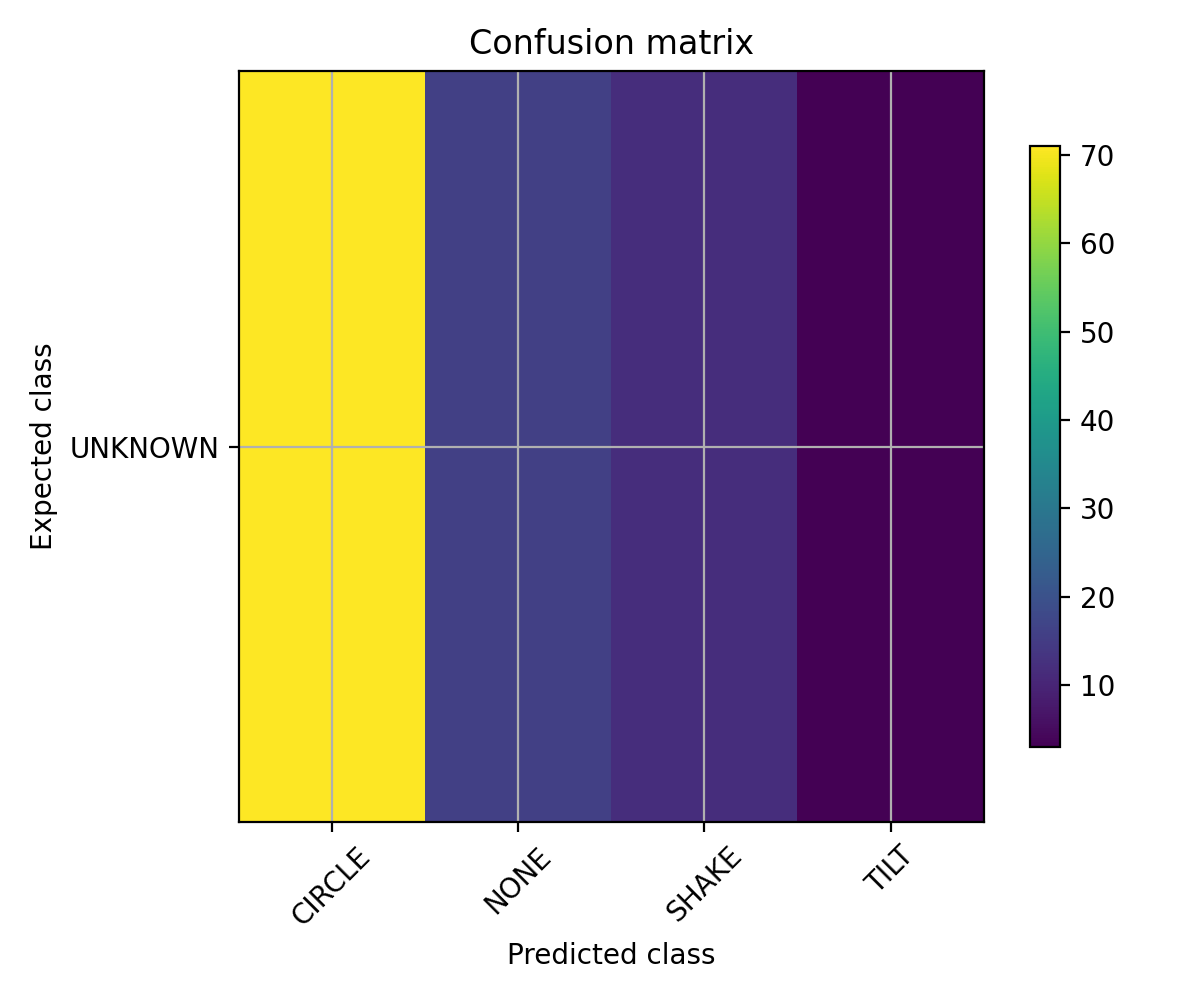
\includegraphics[width=0.9\columnwidth]{figures/confusion_matrix.png}
    \caption{Optional confusion matrix when ground-truth labels are available.}
    \label{fig:confusion}
\end{figure}

\end{document}
